%!TEX root = ../main.tex

\section{Tree-Like Unraveling}\label{sec:unraveling}
We will now describe the construction of the companion structures required in \cref{thm:main-technical-thm}.
Let $\str{A}$ be a structure with an associated binary relation $\relNext \subseteq A \times A$.
A \emph{parent} of an element $e \in A$ is an element $p_{e} \in A$ such that $(p_{e}, e) \in A$.
A \emph{root} is an element which has no parents.
The structure $\str{A}$ is a \emph{forest} if every element has at most one parent and there is at least one root.
A \emph{tree} is a forest with exactly one root.
Using the well-known unraveling for transation systems, it can be shown that every satisfiable modal logic formula is satisfiable in a tree model.
The same holds true for \FGF-formula, using the HAF-unraveling introduced by Bednarczyk~\cite[Sec 3.3]{Bednarczyk21}.
Even though the tree unraveling of a structure $\str{A}, \elemtuplea$ can be infinite for finite $\str{A}$,
for many modal logic variants, companions for a van Benthem style characterisation can be constructed based on the infinite unraveling~\cite{Otto04}.

Unfortuntately, constructing a finite version of the HAF-unraveling is not enough to prove \cref{thm:main-technical-thm}.
Consider the two finite structures shown in \cref{fig:unravel-haf}, which are both already fully HAF-unraveled, but can be distinguished by the GF sentence $\forall b,c. E(b,c) \implies \exists a. P(a,b,c)$.
This shows that even if the HAF-unraveling is finite, it does not provide GF-bisimilar companions.
\begin{figure}
  \centering
    \begin{tikzpicture}[baseline=(current bounding box.north)]
        \draw[tolbrightGreen, line cap=round, line width=2em] (-0em,8em) -- ++(0,-8em);
        \draw[tolbrightYellow, line cap=round, line width=0.5em, -{Latex[length=2em]}] (0,4em) -- (0,0em);

        \draw [black, line width=0.1em, fill=white] (0em, 8em) circle [radius=0.8em] node[anchor=center] {1};
        \draw [black, line width=0.1em, fill=white] (0em, 4em) circle [radius=0.8em] node[anchor=center] {2};
        \draw [black, line width=0.1em, fill=white] (0em, 0em) circle [radius=0.8em] node[anchor=center] {3};

        \begin{scope}[xshift=10em]
            \draw[tolbrightGreen, line cap=round, line width=2em] (-0em,8em) -- ++(0,-8em);
            \draw[tolbrightYellow, line cap=round, line width=0.5em, -{Latex[length=2em]}] (0em,4em) -> (6em,2em);
            \draw[tolbrightYellow, line cap=round, line width=0.5em, -{Latex[length=2em]}] (0,4em) -- (0,0em);

            \draw [black, line width=0.1em, fill=white] (0em, 8em) circle [radius=0.8em] node[anchor=center] {1};
            \draw [black, line width=0.1em, fill=white] (0em, 4em) circle [radius=0.8em] node[anchor=center] {2};
            \draw [black, line width=0.1em, fill=white] (0em, 0em) circle [radius=0.8em] node[anchor=center] {3};
            \draw [black, line width=0.1em, fill=white] (6em, 2em) circle [radius=0.8em] node[anchor=center] {3'};

            \node[tolbrightGreen] at (-2em, 6em) {P};
            \node[tolbrightYellow] at (-1.5em, 2em) {E};
            \node[tolbrightYellow] at (3em, 4em) {E};
        \end{scope}

        \node[font=\Large] at (5em, 4em) {$\sim_{FGF}$};

        \node[tolbrightGreen] at (-2em, 6em) {P};
        \node[tolbrightYellow] at (-1.5em, 2em) {E};
    \end{tikzpicture}%
    \caption{Two FGF-bisimilar HAFs which are not GF-bisimilar. Relations are drawn top to bottom, so the green area marks the relation $\relP(1,2,3)$}%
    \label{fig:unravel-haf}
\end{figure}
We construct an unraveling that fulfills the following theorem:
\begin{theorem}
  Let $\str{A}, \elemtuplea \bisimto_{\FGF} \str{B}, \elemtupleb$ for two pointed $\sigma$-structures.
  Then there are unravelings $\unravel{A}, \elemtuptuplea$ and $\unravel{B}, \elemtuptupleb$ which are both:
  \begin{itemize}
    \item $\FGF$-similar to the original structures: $\unravel{A}, \elemtuptuplea \bisimto_{\FGF} \str{A}, \elemtuplea$ and $\unravel{B}, \elemtuptupleb \bisimto_{\FGF} \str{B}, \elemtupleb$
    \item $\GF$-bisimilar: $\unravel{A}, \elemtuptuplea \bisimto_{\GF} \unravel{B}, \elemtuptupleb$
  \end{itemize}
\end{theorem}

Let $\str{A}, \elemtuplea^{(0)}$ be a pointed $\sigma$-structure.
A \emph{bisimulation sequence} of length $\ell$ is a sequence of the form $\elemtuplea^{(0)}(i^{(1)}, j^{(1)})\elemtuplea^{(1)}\cdots(i^{(\ell)}, j^{(\ell)})\elemtuplea^{(\ell)}$, where each $a^{(k)}$ is a live tuple in $\str{A}$ and $i^{(k)}, j^{(k)}$ are indices such that $\elemtupleafromto{i^{(k)}}{j^{(k)}}^{(k-1)} = \elemtupleafromto{1}{j^{(k)}-i^{(k)}+1}^{k}$.
These bisimulation sequences arise naturally when considering bisimilar structures to $\str{A}$.
If $\str{B}, \elemtupleb^{(0)}$ is a $\sigma$-structure that is \FGF-bisimilar to $\str{A}, \elemtuplea^{(0)}$, then we can apply \ref{bisim:fforth} $\ell$ times to find tuples $\elemtupleb^{1}, \ldots, \elemtupleb^{\ell}$ for a corresponding bisimulation sequence in $\str{B}$.
Note that the infix selected by the indices $(i^{(k)}, j^{(k)})$ is not required to be maximal.
This is illustrated in the following examples of bisimulation sequences.
\begin{figure}[H]
  \centering
    \begin{minipage}[t]{0.2\textwidth}
        \raggedleft
        \vspace{0pt}
        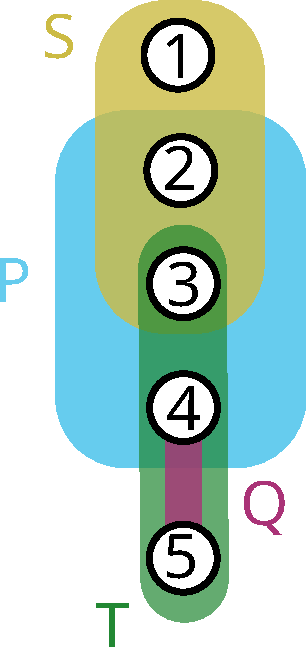
\includegraphics[scale=0.5]{res/example-struct-1}
    \end{minipage}
    \hspace{4em}
    \begin{minipage}[t]{0.6\textwidth}
      {%
      \newcommand{\tups}{{\color{tolbrightYellowDarker}\elemtuples}}%
      \newcommand{\tupp}{{\color{tolbrightCyanDarker}\elemtuplep}}%
      \newcommand{\tupt}{{\color{tolbrightGreen}\elemtuplet}}%
      \newcommand{\tupq}{{\color{tolbrightPurple}\elemtupleq}}%
      The picture on the left shows a structure with the relations: $\relS(1,2,3)$, $\relP(2,3,4)$, $\relT(3,4,5)$, $\relQ(4,5)$

      \vspace{1ex}
      Let $\tups = (1, 2, 3), \tupp = (2, 3, 4), \tupt = (3, 4, 5), \tupq = (4,5)$.

      \vspace{1ex}
      Some examples of bisimulation sequences in this structure are:
      \begin{itemize}
          \item $\tups(3,3)\tupt$
          \item $\tups(2,3)\tupp(2,3)\tupt$
      \end{itemize}

      Bisimulation sequences are not required to use maximal infixes, so the following are also valid bisimulation sequences:
      \begin{itemize}
          \item $\tups(2,2)\tupp$
          \item $\tups(3,3)\tupt(2,2)\tupq$
      \end{itemize}
      }
    \end{minipage}
    \caption{Examples for bisimulation sequences}
\end{figure}

Each tuple in a bisimulation sequence has a prefix of elements which are shared with the preceding tuple, and following this prefix some ``new'' elements which are not shared.
Let $\Seq{A}$ be the set of bisimulation sequences for a structure $\str{A}$.
The \emph{unraveling domain} for the structure $\str{A}$ is defined as the following set:
\bfside{This looks really ugly. Any way to write this in a better way?}
\begin{equation*}
\unraveldom{A} = \Seq{A} \times \mathbb{N} \setminus \left\{ (\sigma(i,j)\bar{a}, k) \colon\, k \le j-i+1\ \text{or}\ k > |a| \right\}
\end{equation*}
For elements $e = (\rho, k) \in \unraveldom{A}$ of this domain, we use the notation $\seq{e} = \rho$ and $\ctr{e} = k$ to refer to the sequence and counter of $e$ respectively.
The element can also be projected into the original structure, using the projection $\pi(e) = \elemtuplea_{k}$ where $\elemtuplea$ is the tuple such that $\rho = \cdots \elemtuplea$. We define the binary relation $\relNext \subseteq \unraveldom{A} \times \unraveldom{A}$ such that $(s, t) \in \relNext$ iff either:
\begin{description}
  \item[(addCtr)] $\seq{s} = \seq{t}$ and $\ctr{t} = \ctr{s} + 1$, or
  \item[(addSeq)] $\seq{t} = \seq{s} (i,j) \elemtuplea$ for some $i, j, \elemtuplea$ and $\ctr{s} = j, \ctr{t} = j - i + 1$
\end{description}
Note that $\unraveldom{A}$ with the relation $\relNext$ is a forest.

% describe finite unraveling
% proof: finite unraveling is FGF-bisimilar to orig structure
% lemma: intersection between any two live tuples is infix
